\section{Day 3: Conditional (Sept 9, 2025)}
In a conditional,
\[
P \to Q
\]
$P$ is called the \textit{antecedent}, and $Q$ is called the \textit{consequent}. The conditional is false if and only if the antecedent is true, yet the consequent is false.

Having `chains' of $\to$ and $\leftrightarrow$ is not a part of official nor informal notation, even though $\leftrightarrow$ commutes with itself. \\

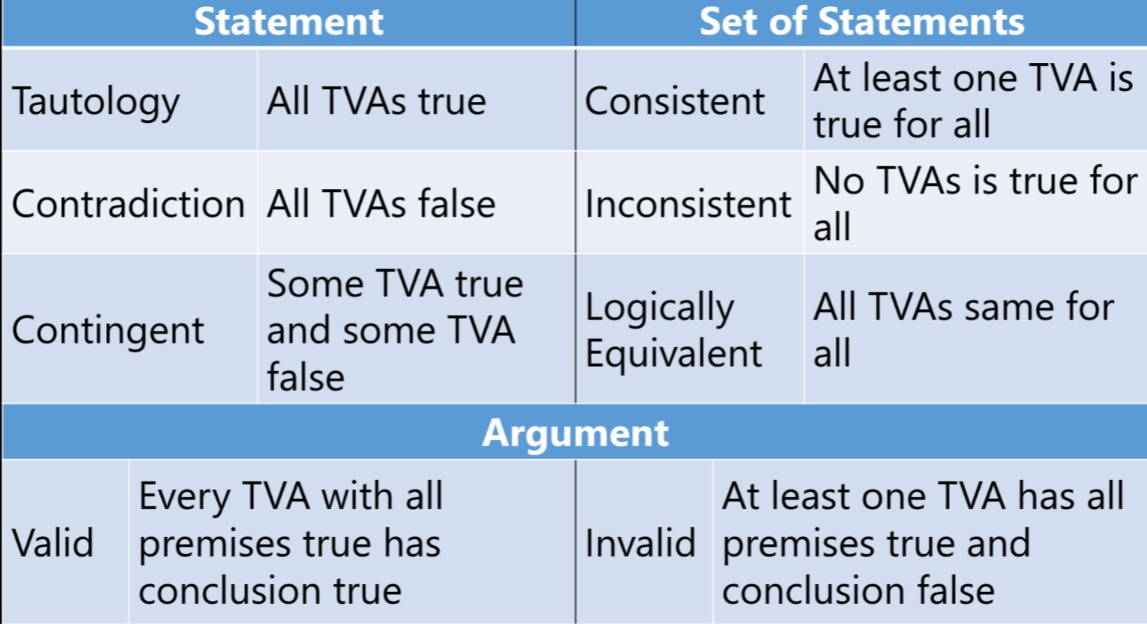
\includegraphics{phl245/figures/sematics.jpg}

\textit{Consistency} and \textit{inconsistency} are properties of sets of statements. \textit{Validity} and its negation are properties of arguments.

\subsection{Truth Tables}
A truth value assignment (TVA) is a row in the truth table, where you try every combination of the atomics' truth values.
